\documentclass[border=5mm]{standalone}
\usepackage{tikz}
\usepackage{amsmath,amssymb}
\usetikzlibrary{arrows.meta,decorations.markings,calc,patterns,shadings,fadings}

% Define colors
% bloch sphere colors
\definecolor{blochpink}{RGB}{220,150,150}
\definecolor{blochred}{RGB}{200,80,80}
% border and panel colors
\definecolor{panelbg}{RGB}{240,240,240}
\definecolor{panelborder}{RGB}{0,80,120}
% atomic cloud colors
\definecolor{atomblue}{RGB}{100,160,220}
\definecolor{atomred}{RGB}{220,130,130}
%misc
\definecolor{arrowred}{RGB}{180,30,30}

\begin{document}
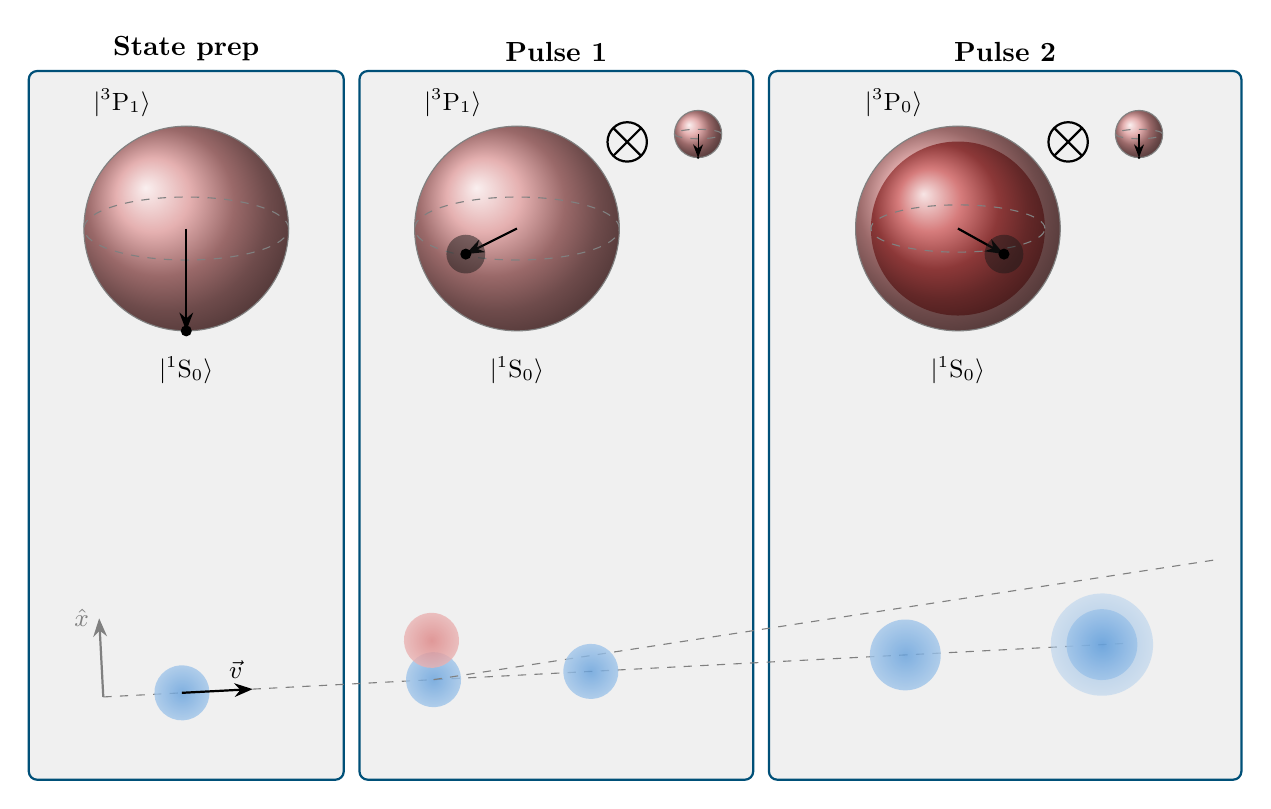
\begin{tikzpicture}[>=Stealth, font=\small]
\def\boxheight{9}
\def\boxgap{0.2}
\def\boxwidtha{4}
\def\boxwidthb{5}
\def\boxwidthc{6}
\def\sphrad{1.3}

% ============================================================
% PANEL 1: State prep
% ============================================================
\begin{scope}[shift={(0,0)}]
  % Background
  \fill[panelbg, rounded corners=3pt] (0,0) rectangle ++(\boxwidtha, \boxheight);
  \draw[panelborder, thick, rounded corners=3pt] (0,0) rectangle ++(\boxwidtha, \boxheight);
  \node[above, font=\bfseries] at (\boxwidtha/2, \boxheight) {State prep};
  % Title
  \begin{scope}[shift={(\boxwidtha/2,\boxheight-2)}]
    % --- Bloch sphere (panel 1) ---
    % Sphere shading
    \shade[ball color=blochpink] (0,0) circle (\sphrad);
    \draw[gray, thin] (0,0) circle (\sphrad);
    % % Equator ellipse
    \draw[gray, dashed, thin] (0,0) ellipse (1.3 and 0.4);
    % % Latitude lines
    % \draw[gray, dotted, thin] (0,0.5) ellipse (1.1 and 0.3);
    % \draw[gray, dotted, thin] (0,-0.5) ellipse (1.1 and 0.3);
    % % State labels
    \node[above left] at (-\sphrad/4,\sphrad) {$|{}^3\text{P}_1\rangle$};
    \node[below] at (0,-1.5) {$|{}^1\text{S}_0\rangle$};
    % Arrow pointing to south pole
    \draw[->,thick] (0,0) -- (0,-\sphrad);
    \fill (0,-\sphrad) circle (2pt);
  \end{scope}
\end{scope}


% ============================================================
% PANEL 2: Pulse 1
% ============================================================
\begin{scope}[shift={(\boxgap+\boxwidtha,0)}]
  % Background
  \fill[panelbg, rounded corners=3pt] (0,0) rectangle ++(\boxwidthb, \boxheight);
  \draw[panelborder, thick, rounded corners=3pt] (0,0) rectangle ++(\boxwidthb, \boxheight);
  \node[above, font=\bfseries] at (\boxwidthb/2, \boxheight) {Pulse 1};
  % Title
  \begin{scope}[shift={(\boxwidthb*0.4,\boxheight-2)}]
    % --- Bloch sphere (panel 1) ---
    % Sphere shading
    \shade[ball color=blochpink] (0,0) circle (\sphrad);
    \draw[gray, thin] (0,0) circle (\sphrad);
    % % Equator ellipse
    \draw[gray, dashed, thin] (0,0) ellipse (1.3 and 0.4);

    % % State labels
    \node[above left] at (-\sphrad/4,\sphrad) {$|{}^3\text{P}_1\rangle$};
    \node[below] at (0,-1.5) {$|{}^1\text{S}_0\rangle$};

    \draw[->,thick] (0,0) -- (-\sphrad*0.5,-\sphrad*0.25);
    \fill[gray!20!black,semitransparent] (-\sphrad*0.5,-\sphrad*0.25) circle (7pt);
    \fill (-\sphrad*0.5,-\sphrad*0.25) circle (2pt);

    % Small circle with X (tensor product / clock symbol) top right
  
    \draw[thick] (1.4,1.1) circle (0.25);
    \draw[thick] (1.4-0.17,1.1+0.17) -- (1.4+0.17,1.1-0.17);
    \draw[thick] (1.4-0.17,1.1-0.17) -- (1.4+0.17,1.1+0.17);

    \begin{scope}[shift={(2.3, 1.2)}]
      \def\sphrad{0.3}
      % --- Bloch sphere (panel 1) ---
      % Sphere shading
      \shade[ball color=blochpink] (0,0) circle (\sphrad);
      \draw[gray, thin] (0,0) circle (\sphrad);
      % % Equator ellipse
      \draw[gray, dashed, thin] (0,0) ellipse (0.3 and 0.06);
      % Arrow pointing to south pole
      \draw[->] (0,0) -- (0,-\sphrad);
      \fill (0,-\sphrad) circle (0.5pt);
    \end{scope}
  \end{scope}
\end{scope}


%============================================================
% PANEL 3: Pulse 2
% ============================================================
\begin{scope}[shift={(\boxgap*2+\boxwidtha+\boxwidthb,0)}]
  % Background
  \fill[panelbg, rounded corners=3pt] (0,0) rectangle ++(\boxwidthc, \boxheight);
  \draw[panelborder, thick, rounded corners=3pt] (0,0) rectangle ++(\boxwidthc, \boxheight);
  \node[above, font=\bfseries] at (\boxwidthc/2, \boxheight) {Pulse 2};
  % Title
  \begin{scope}[shift={(\boxwidthc*0.4,\boxheight-2)}]
    % --- Bloch sphere (panel 3) ---
    % Sphere shading
    
    \shade[ball color=blochpink] (0,0) circle (\sphrad);
    \shade[ball color=blochred] (0,0) circle (\sphrad*0.85);
    
    \draw[gray, thin] (0,0) circle (\sphrad);
    % % Equator ellipse
    \draw[gray, dashed, thin] (0,0) ellipse (\sphrad*0.85 and 0.3);

    % % State labels
    \node[above left] at (-\sphrad/4,\sphrad) {$|{}^3\text{P}_0\rangle$};
    \node[below] at (0,-1.5) {$|{}^1\text{S}_0\rangle$};

    \draw[->,thick] (0,0) -- (+\sphrad*0.45,-\sphrad*0.25);
    \fill[gray!20!black,semitransparent] (+\sphrad*0.45,-\sphrad*0.25) circle (7pt);
    \fill (\sphrad*0.45,-\sphrad*0.25) circle (2pt);

    % Small circle with X (tensor product / clock symbol) top right
  
    \draw[thick] (1.4,1.1) circle (0.25);
    \draw[thick] (1.4-0.17,1.1+0.17) -- (1.4+0.17,1.1-0.17);
    \draw[thick] (1.4-0.17,1.1-0.17) -- (1.4+0.17,1.1+0.17);

    \begin{scope}[shift={(2.3, 1.2)}]
      \def\sphrad{0.3}
      % --- Bloch sphere (panel 1) ---
      % Sphere shading
      \shade[ball color=blochpink] (0,0) circle (\sphrad);
      \draw[gray, thin] (0,0) circle (\sphrad);
      % % Equator ellipse
      \draw[gray, dashed, thin] (0,0) ellipse (0.3 and 0.06);
      % Arrow pointing to south pole
      \draw[->] (0,0) -- (0,-\sphrad);
      \fill (0,-\sphrad) circle (0.5pt);
    \end{scope}
  \end{scope}
\end{scope}


% --- Atom trajectory (panel 1) ---
% x axis
\begin{scope}[rotate=3,shift={(1, 1)}]
  \draw[->, gray, thick] (0,0) -- ++(0, 1) node[left] {$\hat{x}$};
  \draw[gray, dashed, thin] (0,0) -- ++(2*\boxgap + \boxwidtha+\boxwidthb+\boxwidthc*0.6, 0);
  % Atom blob at initial position
  \shade[inner color=atomblue, outer color=atomblue!60!white, opacity=0.8] (1.0,0) circle (0.35);
  
  \shade[inner color=atomblue, outer color=atomblue!60!white, opacity=0.8] (1.0 + 0.8*\boxwidtha ,0) circle (0.35);
  \shade[inner color=atomred, outer color=atomred!60!white, opacity=0.8] (1.0 + 0.8*\boxwidtha , 0.5) circle (0.35);
  \draw[gray, dashed, thin] (1.0 + 0.8*\boxwidtha ,0) -- ++(10, 1) ;

  
  \shade[inner color=atomblue, outer color=atomblue!60!white, opacity=0.8] (1.0 + 1.3*\boxwidtha,0) circle (0.35);
  \shade[inner color=atomblue, outer color=atomblue!60!white, opacity=0.8] (1.0 + \boxwidthb + \boxgap+ \boxwidtha,0) circle (0.45);
  \shade[inner color=atomblue, outer color=atomblue!60!white, opacity=0.8] (1.0 + \boxwidthb*1.5 + \boxgap+ \boxwidtha,0) circle (0.45);
  \shade[inner color=atomblue, outer color=atomblue!50!white, opacity=0.5] (1.0 + \boxwidthb*1.5 + \boxgap+ \boxwidtha,0) circle (0.65);

  
  \draw[->, thick] (1.0,0) -- ++(0.9,0) node[above left] {$\vec{v}$};
\end{scope}

% ============================================================
% PANEL 2: Sequential excitation (first pulse)
% ============================================================
% \begin{scope}[shift={(4.5,0)}]
%   % Background
%   \fill[panelbg, rounded corners=3pt] (-0.3,-4.8) rectangle (4.8,4.5);
%   \draw[panelborder, thick, rounded corners=3pt] (-0.3,-4.8) rectangle (4.8,4.5);

%   % Title (shared with panel 3)
%   \node[above, font=\bfseries] at (5.05,4.5) {Sequential excitation};

%   % --- Bloch sphere (panel 2) ---
%   \begin{scope}[shift={(1.75,2.2)}]
%     % Sphere with partial excitation
%     \shade[ball color=blochpink, opacity=0.35] (0,0) circle (1.3);
%     % Red shading on upper hemisphere for partial excitation
%     \shade[inner color=blochred, outer color=blochpink, opacity=0.4] (0,0.3) circle (0.8);
%     \draw[gray, thin] (0,0) circle (1.3);
%     \draw[gray, dashed, thin] (0,0) ellipse (1.3 and 0.4);
%     \draw[gray, dotted, thin] (0,0.5) ellipse (1.1 and 0.3);
%     \draw[gray, dotted, thin] (0,-0.5) ellipse (1.1 and 0.3);
%     % State labels
%     \node[above left] at (-0.9,1.1) {$|{}^3\text{P}_1\rangle$};
%     \node[below right] at (0.2,-0.7) {${}^1\text{S}_0$};
%     % Small circle with X (tensor product / clock symbol) top right
%     \draw (1.6,1.3) circle (0.25);
%     \draw (1.6-0.17,1.3+0.17) -- (1.6+0.17,1.3-0.17);
%     \draw (1.6-0.17,1.3-0.17) -- (1.6+0.17,1.3+0.17);
%   \end{scope}

%   % --- Atom trajectory (panel 2) ---
%   % Atom blobs showing superposition
%   \shade[inner color=atomblue, outer color=atomblue!10!white, opacity=0.6] (0.8,-3.0) circle (0.3);
%   \shade[inner color=atomblue!50, outer color=white, opacity=0.3] (0.8,-3.0) circle (0.5);
%   % Second blob (excited component, slightly separated)
%   \shade[inner color=atomred, outer color=atomred!10!white, opacity=0.5] (1.5,-2.7) circle (0.25);
%   \shade[inner color=atomblue, outer color=atomblue!10!white, opacity=0.5] (2.2,-2.5) circle (0.25);
%   % Trajectory dashed line
%   \draw[gray, dashed, thin] (-0.3,-3.3) -- (4.8,-1.8);

%   % Laser arrow (k vector)
%   \draw[->, arrowred, ultra thick] (1.5,-3.8) -- (2.8,-3.3);
%   \node[below, text=arrowred, font=\bfseries] at (2.3,-3.9) {$\vec{k}$};

%   % Time label
%   \node[below, font=\large] at (2.25,-4.8) {$t_a$};
% \end{scope}

% ============================================================
% PANEL 3: Sequential excitation (second pulse)
% ============================================================
% \begin{scope}[shift={(9.8,0)}]
%   % Background
%   \fill[panelbg, rounded corners=3pt] (-0.3,-4.8) rectangle (5.3,4.5);
%   \draw[panelborder, thick, rounded corners=3pt] (-0.3,-4.8) rectangle (5.3,4.5);

%   % --- Bloch sphere (panel 3) ---
%   \begin{scope}[shift={(1.75,2.2)}]
%     % Sphere with more excitation (larger red region)
%     \shade[ball color=blochpink, opacity=0.3] (0,0) circle (1.3);
%     \shade[inner color=blochred, outer color=blochpink, opacity=0.6] (0,0.1) circle (1.1);
%     \draw[gray, thin] (0,0) circle (1.3);
%     \draw[gray, dashed, thin] (0,0) ellipse (1.3 and 0.4);
%     % State labels
%     \node[above left] at (-0.8,1.1) {$|{}^3\text{P}_0\rangle$};
%     \node[below] at (0,-1.55) {$|{}^1\text{S}_0\rangle$};
%     % Clock symbol
%     \draw (1.6,1.3) circle (0.25);
%     \draw (1.6-0.17,1.3+0.17) -- (1.6+0.17,1.3-0.17);
%     \draw (1.6-0.17,1.3-0.17) -- (1.6+0.17,1.3+0.17);
%   \end{scope}

%   % --- Atom trajectory (panel 3) ---
%   % Multiple blobs showing wavepacket spreading
%   \shade[inner color=atomblue, outer color=atomblue!10!white, opacity=0.4] (1.0,-2.2) circle (0.25);
%   \shade[inner color=atomred, outer color=atomred!10!white, opacity=0.5] (1.8,-2.0) circle (0.3);
%   \shade[inner color=atomblue, outer color=atomblue!10!white, opacity=0.5] (2.6,-1.7) circle (0.3);
%   \shade[inner color=atomred, outer color=atomred!10!white, opacity=0.5] (3.5,-1.4) circle (0.35);
%   \shade[inner color=atomblue, outer color=atomblue!10!white, opacity=0.6] (4.3,-1.1) circle (0.3);
%   % Trajectory dashed line
%   \draw[gray, dashed, thin] (-0.3,-2.5) -- (5.3,-0.7);
%   % y label
%   \node[right, gray] at (5.0,-0.9) {$y$};

%   % Laser arrow (-k vector, pointing left)
%   \draw[->, arrowred, ultra thick] (3.0,-2.8) -- (1.7,-3.3);
%   \node[above, text=arrowred, font=\bfseries] at (2.5,-2.6) {$-\vec{k}$};

%   % Superposition state label
%   \node[right, font=\small] at (2.5,-3.8) {$|{}^1\text{S}_0\rangle + e^{i\Phi}|{}^3\text{P}_0\rangle$};

%   % Time label
%   \node[below, font=\large] at (2.5,-4.8) {$t_b$};
% \end{scope}

% % ============================================================
% % Time axis
% % ============================================================
% \draw[->, thick, gray] (14.5,-4.8) -- (15.8,-4.8) node[right] {Time};

% ============================================================
% Phase equation at bottom
% ============================================================
% \node[below, font=\normalsize] at (7.5,-5.5) {%
%   $\Phi = \vec{k}\cdot(\vec{r}_0 + \vec{v}\,t_a) + \phi_a
%   - \omega_e(t_b - t_a)
%   - \vec{k}\cdot(\vec{r}_0 + \vec{v}\,t_b) + \phi_b$
% };

\end{tikzpicture}
\end{document}